\section*{Part D: IS-MOS Capacitance}
\addcontentsline{toc}{section}{Part D: IS-MOS Capacitance}

\paragraph{Task 4 a) Labelling and characteristic parameters.}
The curve is a low-frequency MOS C--V on a \textbf{$p$-type substrate}: at negative $V_G$ holes
accumulate ($C=C'_{\max}=C_{ox}$), the capacitance dips through depletion to $C'_{\min}$, and at
positive $V_G$ the low-frequency minority response brings it back up. The three red parameters are
the accumulation plateau $C'_{\max}$, the flat-band value $C'_{FB}$ (the marked point), and the
inversion minimum $C'_{\min}$; the axes are $V_G$ (horizontal) and $C'$ (vertical), see
Fig.~\ref{fig:cv-annot}.

\begin{figure}[H]
\centering
% TikZ overlay on the real docx Figure 3 (Task 4a): fills the blank boxes.
\begin{tikzpicture}
\node[anchor=south west,inner sep=0] (img) at (0,0)
  {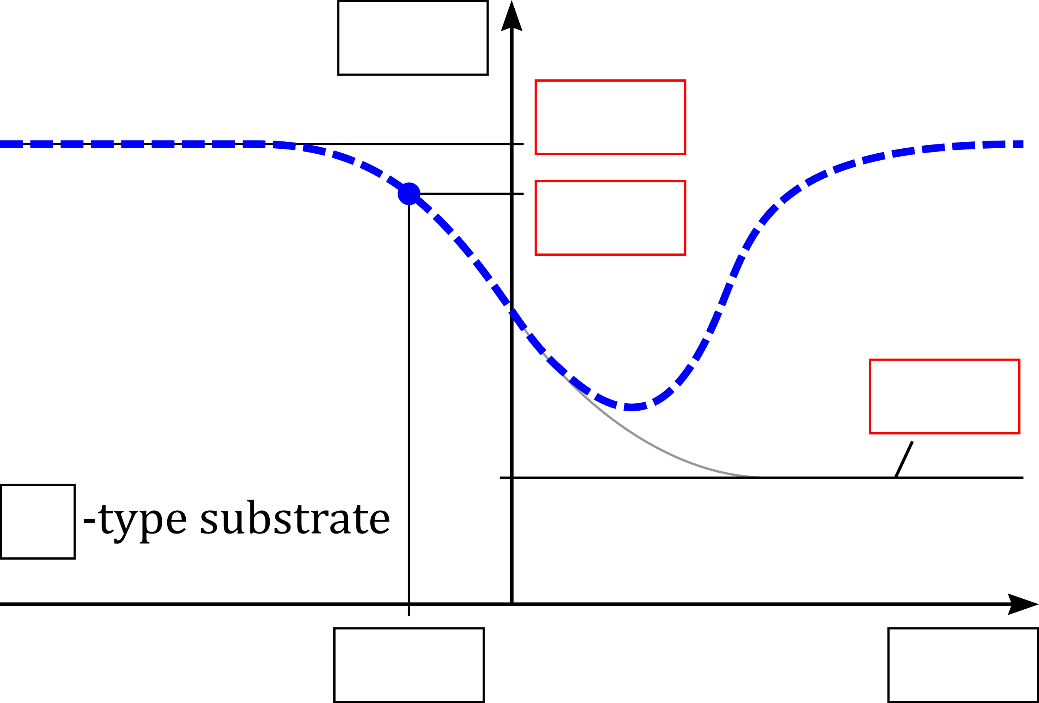
\includegraphics[width=0.66\textwidth]{figures/cv_fig3_blank.png}};
\begin{scope}[x={(img.south east)},y={(img.north west)}]
  \node at (0.385,0.955) {\small $C'$};
  \node at (0.585,0.840) {\scriptsize $C'_{\max}\!=\!C_{ox}$};
  \node at (0.585,0.695) {\scriptsize $C'_{FB}$};
  \node at (0.905,0.445) {\scriptsize $C'_{\min}$};
  \node at (0.035,0.280) {\small $p$};
  \node at (0.385,0.060) {\small $V_{FB}$};
  \node at (0.915,0.060) {\small $V_G$};
\end{scope}
\end{tikzpicture}

\caption{Assignment Figure~3 with the gaps filled in: $p$-type substrate, $y$-axis $C'$ and $x$-axis
$V_G$, the flat-band voltage $V_{FB}$, and the three red parameters $C'_{\max}=C_{ox}$, $C'_{FB}$ and
$C'_{\min}$.}
\label{fig:cv-annot}
\end{figure}

\textbf{(i) Values at \SI{300}{\kelvin}} (SiO$_2$, $\epsilon_r=3.9$, $t_{ox}=\SI{30}{\nm}$;
Si, $\epsilon_r=11.7$, $N=\SI{3e16}{\per\cubic\cm}$). All values per unit area:
\[
C'_{ox}=\frac{\epsilon_{ox}}{t_{ox}}=\SI{1.15e-3}{\farad\per\square\meter}\;(\SI{115}{\nano\farad\per\square\cm}).
\]
The bulk potential is $\phi_F=\tfrac{k_BT}{e}\ln\!\tfrac{N}{n_i}=\SI{0.375}{\volt}$, giving a maximum
depletion width
$W_{\max}=\sqrt{4\epsilon_{Si}\phi_F/(eN)}=\SI{180}{\nm}$ and Debye length
$L_D=\sqrt{\epsilon_{Si}(k_BT/e)/(eN)}=\SI{23.6}{\nm}$. With
$C'_{\min}=C_{ox}C_{sc}/(C_{ox}+C_{sc})$ for each series semiconductor capacitance:
\begin{center}\small
\begin{tabular}{lccc}
\toprule
Gate / doping & $C'_{\max}=C_{ox}$ & $C'_{FB}$ & $C'_{\min}$ \\
 & [nF/cm$^2$] & [nF/cm$^2$] & [nF/cm$^2$] \\
\midrule
SiO$_2$, $N=3{\times}10^{16}$ & 115 & 91 & 38.4 \\
\bottomrule
\end{tabular}
\end{center}

\textbf{(ii) Si$_3$N$_4$ gate ($\epsilon_r=7.5$) and lower doping $N=\SI{0.5e16}{\per\cubic\cm}$.}
The higher-$\kappa$ oxide nearly doubles $C_{ox}$, and the lighter doping widens the depletion region
($W_{\max}=\SI{413}{\nm}$), lowering $C'_{\min}$:
\begin{center}\small
\begin{tabular}{lccc}
\toprule
Gate / doping & $C'_{\max}$ & $C'_{FB}$ & $C'_{\min}$ \\
 & [nF/cm$^2$] & [nF/cm$^2$] & [nF/cm$^2$] \\
\midrule
Si$_3$N$_4$, $N=0.5{\times}10^{16}$ & 221 & 99 & 22.6 \\
\bottomrule
\end{tabular}
\end{center}
The capacitance swing grows from $C_{\max}-C_{\min}=\SI{77}{\nano\farad\per\square\cm}$ to
\SI{199}{\nano\farad\per\square\cm}, a factor of $2.6$. With $\Delta V$ fixed, the slope
$\Delta C/\Delta V$ therefore rises by the same factor, so the change makes a
\textbf{more sensitive sensor}.

\paragraph{Task 4 b) C--V modifications (low frequency).}
The flat-band voltage is
$V_{FB}=\tfrac{\phi_M}{e}-\tfrac{\phi_{Si}}{e}-\tfrac{Q_{ox}+Q_{ss}}{C_{ox}}$ (EOS adds
$E_{REF}-\psi_0+\chi_{sol}$). Each effect shifts the curve horizontally without changing its shape
(Fig.~\ref{fig:cv-mods}):
\begin{itemize}[nosep,leftmargin=1.4em]
\item \textbf{(i)} Fixed positive $Q_{ox},Q_{ss}$ lower $V_{FB}$ $\Rightarrow$ shift to the
\textbf{left} (negative $V$).
\item \textbf{(ii)} A higher semiconductor work function $\phi_{Si}$ also lowers $V_{FB}$
$\Rightarrow$ shift \textbf{left}.
\item \textbf{(iii)} Increasing pH makes $\psi_0$ more negative, and since $V_{FB}$ contains
$-\psi_0$ the curve shifts to the \textbf{right} ($\le\SI{59}{\milli\volt}/\mathrm{pH}$).
\end{itemize}

\begin{figure}[H]
\centering
% Auto-generated: TikZ overlay on the real docx Figure 4 (Task 4b)
\begin{tikzpicture}
\node[anchor=south west,inner sep=0] (img) at (0,0)
  {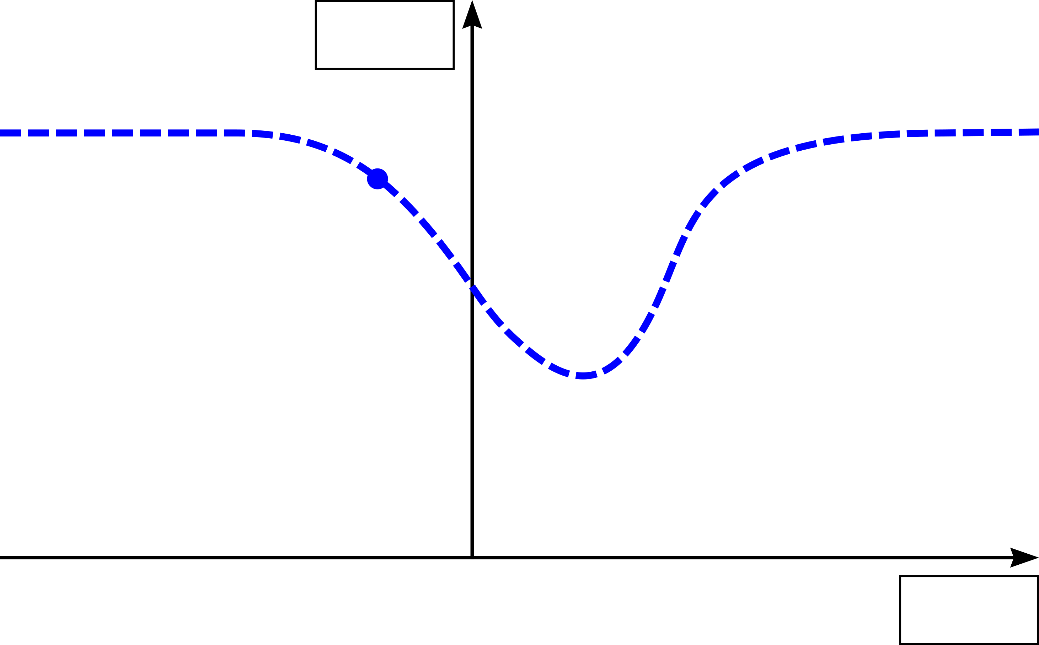
\includegraphics[width=0.66\textwidth]{figures/cv_fig4_blank.png}};
\begin{scope}[x={(img.south east)},y={(img.north west)}]
  \clip (0.0,0.13) rectangle (1.0,0.97);
  \draw[red,dashed,line width=1.1pt] plot coordinates {(0.000,0.795) (0.029,0.795) (0.059,0.795) (0.096,0.795) (0.125,0.794) (0.154,0.788) (0.182,0.777) (0.209,0.759) (0.234,0.729) (0.257,0.705) (0.281,0.671) (0.304,0.622) (0.328,0.572) (0.351,0.517) (0.374,0.478) (0.398,0.445) (0.424,0.423) (0.452,0.420) (0.481,0.455) (0.504,0.505) (0.527,0.586) (0.550,0.665) (0.575,0.716) (0.601,0.743) (0.629,0.763) (0.657,0.775) (0.686,0.784) (0.715,0.789) (0.745,0.793) (0.782,0.795) (0.812,0.795) (0.842,0.795) (0.871,0.796) (1.000,0.796)};
  \draw[green!55!black,dash dot,line width=1.1pt] plot coordinates {(0.000,0.795) (0.030,0.795) (0.059,0.795) (0.089,0.795) (0.119,0.795) (0.156,0.795) (0.185,0.794) (0.214,0.788) (0.242,0.777) (0.269,0.759) (0.294,0.729) (0.317,0.705) (0.341,0.671) (0.364,0.622) (0.388,0.572) (0.411,0.517) (0.434,0.478) (0.458,0.445) (0.484,0.423) (0.512,0.420) (0.541,0.455) (0.564,0.505) (0.587,0.586) (0.610,0.665) (0.635,0.716) (0.661,0.743) (0.689,0.763) (0.717,0.775) (0.746,0.784) (0.775,0.789) (0.805,0.793) (0.842,0.795) (0.872,0.795) (0.902,0.795) (0.931,0.796) (1.000,0.796)};
  \draw[violet,densely dotted,line width=1.1pt] plot coordinates {(0.000,0.795) (0.120,0.795) (0.150,0.795) (0.180,0.795) (0.210,0.795) (0.239,0.795) (0.269,0.795) (0.299,0.795) (0.336,0.795) (0.365,0.794) (0.394,0.788) (0.422,0.777) (0.449,0.759) (0.474,0.729) (0.497,0.705) (0.521,0.671) (0.544,0.622) (0.568,0.572) (0.591,0.517) (0.614,0.478) (0.638,0.445) (0.664,0.423) (0.692,0.420) (0.721,0.455) (0.744,0.505) (0.767,0.586) (0.790,0.665) (0.815,0.716) (0.841,0.743) (0.869,0.763) (0.897,0.775) (0.926,0.784) (0.955,0.789) (0.985,0.793) (1.000,0.793)};
  \draw[red,-{Latex},line width=0.9pt] (0.40,0.66)--(0.31,0.66);
  \draw[violet,-{Latex},line width=0.9pt] (0.62,0.66)--(0.71,0.66);
\end{scope}
\begin{scope}[x={(img.south east)},y={(img.north west)}]
  \node at (0.37,0.915) {\small $C$};
  \node at (0.93,0.05) {\small $V_G$};
\end{scope}
\end{tikzpicture}

\caption{Sketched over assignment Figure~4 (blue = ideal). \textcolor{red}{(i) red, dashed}: positive
fixed charge shifts left; \textcolor{green!55!black}{(ii) green, dash-dot}: higher work function
shifts left; \textcolor{violet}{(iii) violet, dotted}: increased pH shifts right.}
\label{fig:cv-mods}
\end{figure}

\paragraph{Task 4 c) EOS-Cap pH sensitivity.}
In the linear regime the chemical sensitivity is the product of the (shared) electrical slope and the
voltage shift per pH, $\Delta C/\Delta\mathrm{pH}=(\Delta C/\Delta V)\,(\Delta V/\Delta\mathrm{pH})$,
with the Nernst limit $\Delta V/\Delta\mathrm{pH}=2.303\tfrac{k_BT}{e}\,\alpha=\SI{59.5}{\milli\volt}\,\alpha$:
\[
\text{A (SiO}_2,\ \alpha=0.5):\ \frac{\Delta V}{\Delta\mathrm{pH}}=\SI{29.8}{\milli\volt}/\mathrm{pH},\qquad
\text{B (Al}_2\text{O}_3,\ \alpha=0.9):\ \frac{\Delta V}{\Delta\mathrm{pH}}=\SI{53.6}{\milli\volt}/\mathrm{pH}.
\]
Because both devices share the same slope $\Delta C/\Delta V$, their capacitive sensitivities scale
the same way: $\boxed{\,(\Delta C/\Delta\mathrm{pH})_B/(\Delta C/\Delta\mathrm{pH})_A=\alpha_B/\alpha_A=1.8\,}$.
The near-Nernstian Al$_2$O$_3$ device is $1.8\times$ more sensitive than the sub-Nernstian SiO$_2$ one.

\paragraph{Task 4 d) Effect of a different semiconductor.}
The pH response lives at the \emph{oxide--electrolyte} interface (it is set by $\psi_0$ and the
site-dissociation chemistry), so the intrinsic sensitivity in mV/pH does \textbf{not} change with the
semiconductor. What does change is the baseline: a different work function $\phi_{Si}$, bandgap, $n_i$
and permittivity shift $V_{FB}$ and reshape the C--V curve (different $C_{\min}$, depletion width) and
alter temperature stability and leakage. In short, the curve moves and rescales, but the pH
slope stays the same.
